%--------------------------------------------------------------------------------
%
%--------------------------------------------------------------------------------
\unnumberedChapter{Controller Dependent Code}

The LCS runtime library already shields the firmware programmer from many of the 
details of the underlying communication protocol. Firmware no longer needs to deal
 with CAN frame formats, node addressing, message dispatching or event handling. 
 However, another source of complexity still remains: the hardware platform itself.

Every hardware module combines a particular controller family with a specific board
design. Besides the processor itself, a typical module contains a CAN bus interface,
non-volatile memory and an extension connector exposing a number of controller 
pins to the outside world. Even when two boards perform the same task, they 
often differ in their pin assignments or make use of different controller 
peripherals. Supporting several board revisions or even different controller 
families would quickly lead to a large amount of controller specific code and 
conditional compilation throughout the firmware.

The \textbf{Controller Dependent Code (CDC)} library addresses this problem by 
concentrating all controller and board specific knowledge into one dedicated 
software layer. The runtime library and the application firmware no longer
access controller peripherals directly. Instead, they operate on abstract hardware
resources that are configured once during system initialization.

The CDC layer deliberately provides only a thin abstraction. It hides the details
that would otherwise clutter the firmware, while still allowing direct access to
the underlying controller whenever this is required. In this way the common 
firmware remains portable without preventing applications from taking advantage
 of controller specific features.

This chapter introduces the concepts behind the CDC library, the resource based
configuration mechanism and the services that are provided to the upper software 
layers.


%--------------------------------------------------------------------------------
\unnumberedSection{Concept}

The CDC library is based on two simple ideas.

The first idea is to separate the description of the hardware from its actual
configuration. Every supported board is described by a constant
\textbf{resource descriptor map}. This description specifies the board type,
board version and the hardware resources available on that board together with
their pin assignments and configuration parameters. Since these descriptions are
constant data structures, adding support for a new board revision normally
requires little more than defining another descriptor map.

During initialization the descriptor map is processed by the CDC library. The
library validates the hardware description, checks that the requested controller
functions are available on the selected pins and creates the internal
\textbf{resource map}. This runtime data structure contains the information
required for efficient access to the configured hardware resources.

The second idea is that firmware should no longer access controller pins or SDK
objects directly. Instead, every configured hardware function is assigned a
\textbf{resource number}. From this point onwards the firmware refers only to
this resource number, independent of the actual controller family or PCB
revision.

This concept is comparable to the use of file handles in an operating system.
Once a file has been opened, applications no longer access the physical storage
device directly but use the file handle returned by the operating system.
Similarly, the CDC library returns resource numbers that uniquely identify the
configured hardware resources.

The resource abstraction is intentionally not limited to simple controller
peripherals such as GPIO pins, timers or serial interfaces. Higher level
resources can also be introduced whenever they simplify firmware development.
For example, a DCC output, an encoder with push button or an H-bridge driver can
be represented as individual resources although internally they consist of
several controller peripherals.

\begin{center}
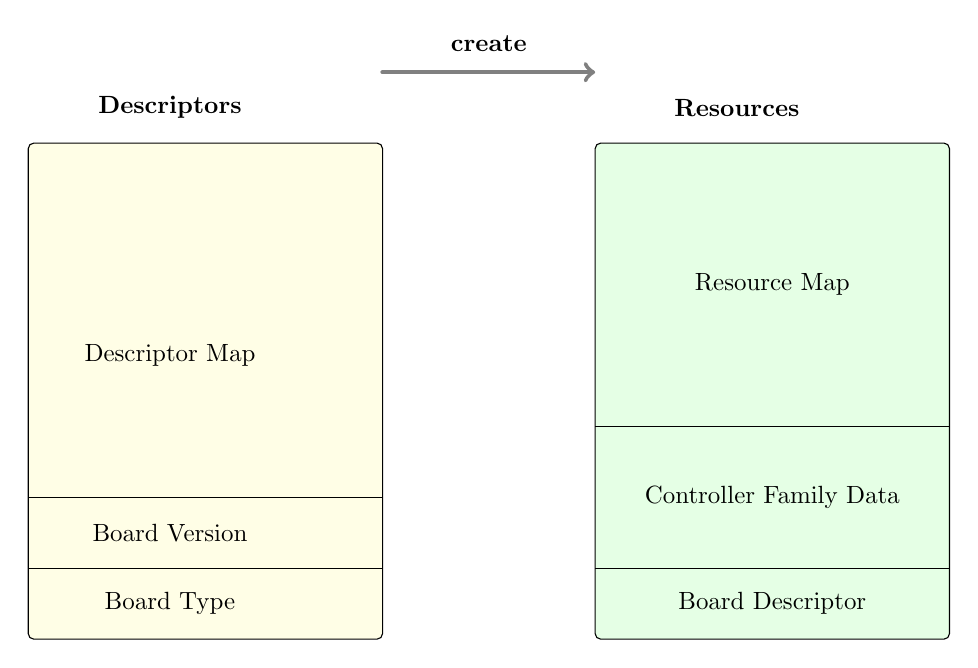
\begin{tikzpicture}[scale=0.9, transform shape]

     % flow
     \node at (8.5,8.4) {\textbf{create}};
     \draw[->, ultra thick, gray, line cap=round] (7,8) -- (10,8);

     % rectangles
     \draw[rounded corners=2pt, fill=yellow!10] (2,0) rectangle (7,7);
     \draw[rounded corners=2pt, fill=green!10] (10,0) rectangle (15,7);

     % Descriptors
     \node at (4,7.5) {\textbf{Descriptors}};
     \node at (4,0.5) {Board Type};
     \draw (2,1)--(7,1);

     \node at (4,1.5) {Board Version};
     \draw (2,2)--(7,2);

     \node at (4,4) {Descriptor Map};

     % Resources
     \node at (12,7.5) {\textbf{Resources}};
     \node at (12.5,0.5) {Board Descriptor};
     \draw (10,1)--(15,1);

     \node at (12.5,2) {Controller Family Data};
     \draw (10,3)--(15,3);

     \node at (12.5,5) {Resource Map};
   
\end{tikzpicture}
\end{center}
\FloatBarrier

During system initialization the resource descriptor map is passed to the CDC
library. The library creates all configured hardware resources and performs the
necessary controller specific initialization. Once this process has completed,
both the runtime library and the application firmware access the hardware
exclusively through the assigned resource numbers.

Using the CDC library does not prevent direct access to the controller hardware.
Whenever an application requires functionality that is not covered by the CDC
abstraction, controller specific SDK routines can still be used directly.
However, such code is naturally less portable between different controller
families.

\paragraph{Why resources instead of pins?}

Traditional embedded software is often written around controller pins and
peripherals. As a consequence, changing the controller family or introducing a
new PCB revision frequently requires modifications throughout the application.
The CDC library reverses this dependency. Applications describe the hardware
resources they require, while the controller specific implementation determines
how these resources are realized on the selected hardware. This approach keeps
the upper software layers almost completely independent of pin assignments,
controller specific SDKs and board revisions.

%--------------------------------------------------------------------------------
\unnumberedSection{CDC Resource Descriptor Map}

The \textbf{Resource Descriptor Map} is the central configuration data structure
of the CDC library. It provides a declarative description of the hardware
available on a particular board. Each supported board type and board revision
has its own descriptor map, which is normally implemented as a constant data
structure residing in program memory.

The descriptor map does not contain any runtime information. Instead, it merely
describes the hardware resources offered by the board. During library
initialization this description is interpreted by the CDC library, which creates
the corresponding runtime resources.

The descriptor map contains three kinds of information:

\begin{itemize}
\item the board type,
\item the board version, and
\item a list of resource descriptors.
\end{itemize}

Each resource descriptor defines one hardware capability together with the
parameters required to configure it. Depending on the resource type, these
parameters may include controller pin assignments, baud rates, timer periods,
PWM frequencies or other controller specific settings.

The descriptor map therefore becomes the \emph{single source of truth} for the
hardware configuration of a particular board. Whenever the board layout changes,
only the corresponding descriptor map needs to be updated. The runtime library
and the application firmware remain completely unchanged.

The descriptor map itself is defined as follows.

\lstset{language=c++, style=codesnippetstyle}
\begin{lstlisting}
struct CdcResourceDescMap {

    uint16_t            boardType;
    uint16_t            boardVersion;
    CdcResourceDesc     map[ MAX_RES_DESC_ENTRIES ];
};
\end{lstlisting}
\FloatBarrier

Each entry of the descriptor array represents one hardware resource. The exact
contents depend on the resource type being described. Since different hardware
resources require different configuration parameters, the resource descriptor
contains a union of resource specific data structures.

For example, a simple GPIO resource only needs to describe the controller pin
assignment together with its operating mode.

\lstset{language=c++, style=codesnippetstyle}
\begin{lstlisting}
struct {

            uint8_t     pinA;
            uint8_t     pinB;
            uint8_t     pinMode;

        } gpio;
\end{lstlisting}
\FloatBarrier

Higher level resources combine pin assignments and settings in one resource. 
As an example here is the I2C  resource descriptor:

\lstset{language=c++, style=codesnippetstyle}
\begin{lstlisting}
struct {

            uint8_t     sclPin;
            uint8_t     sdaPin;
            uint32_t    baudRate;
            uint32_t    i2cTimeoutMs; 

        } i2c;
\end{lstlisting}
\FloatBarrier

For each board and version there is a resource map, describing the actual hardware.
 During configuration this data is used to build the \textbf{Resource Map}. 

%--------------------------------------------------------------------------------
\unnumberedSection{CDC Resource Map}

While the Resource Descriptor Map is a static description of the hardware, the
\textbf{Resource Map} contains the runtime representation created by the CDC
library during initialization.

For every descriptor contained in the descriptor map, the corresponding
configuration routine validates the requested hardware configuration, initializes
the controller peripheral and creates an internal resource entry. These runtime
entries are subsequently used by all CDC service routines.

The Resource Map therefore represents the configured hardware rather than its
description.

A key concept is that every configured resource receives a unique
\textbf{Resource Number}. This number serves as the handle by which the resource
is referenced throughout the lifetime of the application.

The concept closely resembles the use of file descriptors in an operating
system. After opening a file, an application no longer refers to the underlying
storage device but simply uses the returned file descriptor. Likewise, firmware
never accesses controller pins directly after initialization. Instead, all CDC
functions operate on Resource Numbers.

Since Resource Numbers are implemented as simple indices into the internal
Resource Map, resource lookup requires only a single array access and therefore
adds virtually no runtime overhead.

\lstset{language=c++, style=api-interface}
\begin{lstlisting}
enum CdcResourceIdNum : uint8_t {

    CDC_RN_ACTIVITY_LED     = 0,
    CDC_RN_PFAIL            = 1,
    CDC_RN_CAN_BUS          = 2,
    CDC_RN_NVM              = 3,
    CDC_RN_EXT_NVM          = 4,
    CDC_RN_RESERVED_1       = 5,
    CDC_RN_RESERVED_2       = 6,
    CDC_RN_RESERVED_3       = 7,
    CDC_RN_FIRST_USER_RN    = 8, 

    CDC_RN_UNDEFINED        = 255
};
\end{lstlisting}
\FloatBarrier

The first Resource Numbers are reserved for the runtime library itself. They
identify resources that are required by every LCS node, such as the activity
LED, the CAN interface or the non-volatile memory.

Application specific resources begin at
\texttt{CDC\_RN\_FIRST\_USER\_RN}. From this point onwards the firmware designer
is free to define resources that best describe the application rather than the
underlying controller peripherals.

Typical examples include encoder interfaces, DCC outputs, H-bridge controllers,
servo drivers or complete occupancy detector channels. Such logical resources
may internally combine several controller peripherals while still presenting a
single, easy-to-use interface to the application firmware.

\paragraph{Configuration Validation}

Besides configuring the controller peripherals, the CDC library performs a
number of consistency checks during initialization. These checks detect many
hardware configuration errors before the application starts executing.

Typical validation includes verifying that the selected controller pins support
the requested peripheral function, ensuring that no hardware resource is
allocated more than once and checking that all required controller capabilities
are available on the selected processor family.

Detecting such problems during system initialization considerably simplifies
debugging and avoids a large class of runtime errors that would otherwise only
be discovered after deployment.

%--------------------------------------------------------------------------------
\unnumberedSection{CDC Library setup}

\lstset{language=c++, style=api-interface}
\begin{lstlisting}
uint8_t         cdcInit( CdcResourceDescMap *dMap, 
                         uint16_t           options = 0, 
                         uint16_t           debugMask = 0 );

CdcResourceDesc *lookupResourceDesc( uint8_t rNum, uint8_t type );
void            printResourceDescMap( CdcResourceDescMap *dMap );
void            printResourceMap( );

uint32_t        getVersion( );
uint32_t        getPatchLevel( );

void            fatalError( uint8_t errNum, 
                            char    *str  = nullptr,  
                            uint8_t rStat = NO_ERR );

uint16_t        getDebugMask( );
void            setDebugMask( uint16_t mask );
\end{lstlisting}
\FloatBarrier

%--------------------------------------------------------------------------------
\unnumberedSection{General Utility Functions}

The CDC library provides a number of utility functions that are independent of
any particular hardware resource. These routines expose general controller
services that are required throughout the LCS software stack.

The timing functions return the elapsed milliseconds or microseconds since
system startup and provide simple delay routines. They are primarily intended
for initialization and low-level timing tasks.

Every controller also provides a unique hardware identifier from which the CDC
library derives a compact serial number or unique node identifier. This
identifier can be used whenever an LCS node requires a hardware unique address
or serial number.

\lstset{language=c++, style=api-interface}
\begin{lstlisting}
uint32_t        getMillis( );
uint32_t        getMicros( );
void            sleepMillis( uint32_t val );
void            sleepMicros( uint32_t val );
uint64_t        getSerialNum( );
uint32_t        createUid( );
\end{lstlisting}
\FloatBarrier

%--------------------------------------------------------------------------------
\unnumberedSection{Console IO}

During development and debugging, console output is one of the most valuable
tools. The CDC library therefore offers a simple console interface that shields
the firmware from the underlying USB implementation.

The interface intentionally resembles the familiar \texttt{printf()} model. On
controllers supporting multiple USB communication channels, individual channels
can be selected independently. Applications can also determine whether a host
terminal is currently connected before attempting to transmit debug messages.

\lstset{language=c++, style=api-interface}
\begin{lstlisting}
uint8_t         configureUsbIO( );
bool            usbIsConnected( );
char            usbIoGetChar( int chan, uint32_t timeoutVal = 0 );            
int             usbIoPrintf( int chan, const char *fmt, ... );
\end{lstlisting}
\FloatBarrier

%--------------------------------------------------------------------------------
\unnumberedSection{Controller Family}

Although the CDC library hides most controller specific details, applications
occasionally need to obtain information about the underlying hardware. This
group of functions provides access to controller capabilities such as processor
family, memory sizes and CPU frequency.

The watchdog interface is likewise implemented in a controller independent
manner. Applications can therefore enable, update and query the watchdog
without depending on the vendor specific SDK.

\lstset{language=c++, style=api-interface}
\begin{lstlisting}
uint8_t         getBoardId( uint16_t *bId );
uint8_t         getControllerFamily( uint16_t *family );
uint8_t         getControllerChip( uint16_t *chip );
uint8_t         getChipMemSize( uint32_t *size );
uint8_t         getChipNvmSize( uint32_t *size );
uint8_t         getChipCpuFrequency( uint32_t *frequency );

uint8_t         watchDogEnable( bool enable );
uint8_t         watchDogUpdate( );
uint8_t         watchDogCausedReboot( bool *reboot );
\end{lstlisting}
\FloatBarrier

%--------------------------------------------------------------------------------
\unnumberedSection{Timer Management}

The runtime library itself does not require a general purpose timer. However,
timers are indispensable for many hardware related applications. DCC signal
generation, software PWM and protocol timing are typical examples.

The CDC timer interface provides repeating timers with callback functions. A
timer period is specified in microseconds and automatically restarts after each
expiration. In addition, the timer period can be modified while the timer is
running without disturbing the current timing cycle. This allows applications to
generate precisely timed signals with very little software overhead.

\lstset{language=c++, style=api-interface}
\begin{lstlisting}
uint8_t         configureTimer( uint8_t rNum, 
                                TimerCallback functionId, 
                                bool highPri = false );

uint8_t         startRepeatingTimer( uint8_t rNum, uint32_t val );
uint8_t         stopRepeatingTimer( uint8_t rNum );
uint8_t         setRepeatingTimerLimit( uint8_t rNum, uint32_t val );
uint8_t         getRepeatingTimerLimit( uint8_t rNum, uint32_t *val );
\end{lstlisting}
\FloatBarrier

%--------------------------------------------------------------------------------
\unnumberedSection{Analog Input}

Analog input resources configure controller pins for analog-to-digital
conversion. Once configured, applications simply reference the corresponding
resource number to obtain the current conversion result.

The CDC interface deliberately hides controller specific ADC numbering and pin
assignment rules, allowing applications to remain independent of the underlying
processor family.

\lstset{language=c++, style=api-interface}
\begin{lstlisting}
uint8_t         configureAdc( uint8_t rNum );
uint8_t         configureAdc( uint8_t rNum, uint8_t adcPin, uint8_t adcNum );
uint8_t         readAdc( uint8_t rNum, uint16_t *val );
\end{lstlisting}
\FloatBarrier

%--------------------------------------------------------------------------------
\unnumberedSection{Digital IO}


The digital IO routines offer an interface to plain digital input and output 
operations. If it is an input channel, the input can be set to active low or high
input. Also, there is an option to enable the controller internal input pull-up 
resistor. For configured output pins, two pins can be set in pairs if supported 
by the actual hardware configuration, i.e. the two IO pins are on the same 
controller output port. This feature enables the simultaneous setting the two
pins. A typical use case is the DCC signal where the two signal levels are set in
one call.

Once configured, digital inputs and outputs are accessed exclusively through
their Resource Number. Firmware therefore remains independent of the actual pin
assignment used by the selected hardware module.

\lstset{language=c++, style=api-interface}
\begin{lstlisting}
uint8_t         configureDio( uint8_t rNum );
uint8_t         configureDio(   uint8_t rNum, 
                                uint8_t pinA, 
                                uint8_t pinB, 
                                uint8_t pinMode );
uint8_t         readDio( uint8_t rNum, bool *valA, bool *valB = nullptr );
uint8_t         writeDio( uint8_t rNum, bool valA, bool valB = false );
uint8_t         toggleDio( uint8_t rNum );
uint8_t         registerDioCallback( uint8_t rNum, 
                                     uint8_t event, 
                                     GpioCallback func );
uint8_t         unregisterDioCallback( uint8_t rNum );

uint8_t         getGpioPinA( uint8_t rNum) ;
uint8_t         getGpioPinB( uint8_t rNum );
\end{lstlisting}
\FloatBarrier

%--------------------------------------------------------------------------------
\unnumberedSection{PWM Output}

Pulse Width Modulation (PWM) is commonly used to control LED brightness, motor
speed or other analog-like output signals. Most controller families provide
hardware PWM units, although their programming models often differ considerably.

The CDC library exposes a uniform PWM interface that hides these controller
specific details. During configuration the appropriate controller resources are
allocated and initialized. Applications subsequently only specify the desired
frequency and duty cycle through the corresponding Resource Number.

Where supported by the controller hardware, paired PWM outputs can be updated
synchronously to avoid unwanted timing skew between the two channels.

\lstset{language=c++, style=api-interface}
\begin{lstlisting}
uint8_t         configurePwm( uint8_t rNum );
uint8_t         configurePwm(   uint8_t rNum, 
                                uint8_t pinA, 
                                uint8_t pinB, 
                                uint32_t frequency );
                                
uint8_t         setPwmFrequency( uint8_t rNum, uint32_t frequency );

uint8_t         writePwm( uint8_t rNum,
                          uint8_t dutyCycleA, 
                          uint8_t dutyCycleB = 0 ); 

uint8_t         syncPwm( uint8_t rNum );
\end{lstlisting}
\FloatBarrier

%--------------------------------------------------------------------------------
\unnumberedSection{Serial IO}

The UART resource provides asynchronous serial communication. Within the LCS
project it is primarily used for RailCom communication, although the interface
is suitable for any asynchronous serial data stream.

Currently the CDC implementation focuses on buffered receive operation, which is
sufficient for the intended applications. The interface has deliberately been
designed so that additional transmit functionality can be added later without
changing the overall programming model.

\lstset{language=c++, style=api-interface}
\begin{lstlisting}
uint8_t         configureUart( uint8_t rNum );
uint8_t         configureUart(  uint8_t rNum, 
                                uint8_t rxPin, 
                                uint8_t txPin, 
                                uint32_t baudRate );
uint8_t         startUartRead( uint8_t rNum );
uint8_t         stopUartRead( uint8_t rNum );
uint8_t         getUartBuffer( uint8_t rNum, uint8_t *buf, uint8_t bufLen );
\end{lstlisting}
\FloatBarrier

%--------------------------------------------------------------------------------
\unnumberedSection{I2C Interface}

The I\textsuperscript{2}C resource encapsulates the complete controller specific
initialization of an I\textsuperscript{2}C bus. Besides configuring the hardware
pins and baud rate, the CDC library also performs validation of the selected pin
assignment where required by the controller family.

Read and write operations are performed through the configured Resource Number,
allowing the application to remain independent of the actual controller
instance. Additional utility functions support bus recovery and automatic device
scanning during development.

\lstset{language=c++, style=api-interface}
\begin{lstlisting}
uint8_t         configureI2C( uint8_t rNum );
uint8_t         configureI2C( uint8_t rNum, 
                              uint8_t sclPin, 
                              uint8_t sdaPin, 
                              uint32_t baudRate, 
                              uint32_t timeOut );

uint8_t         i2cBusreset( uint8_t rNum );

uint8_t         i2cWrite( uint8_t  rNum, 
                          uint8_t  i2cAdr, 
                          uint8_t  *buf, 
                          uint16_t len, 
                          bool     stopBit );

uint8_t         i2cRead( uint8_t  rNum,
                         uint8_t  i2cAdr, 
                         uint8_t  *buf, 
                         uint16_t len, 
                         bool     stopBit = false );

uint8_t         i2cGetSclPin( uint8_t rNum );
uint8_t         i2cGetSdaPin( uint8_t rNum );
uint8_t         i2cGetBaudrate( uint8_t rNUm );
uint8_t         scanI2CBus( uint8_t rNum );
\end{lstlisting}
\FloatBarrier

%--------------------------------------------------------------------------------
\unnumberedSection{CAN Interface}

The CAN resource provides the communication channel used by the LCS runtime
library. Depending on the controller family, the implementation may either use a
dedicated CAN controller or emulate CAN functionality using programmable
hardware such as the Raspberry Pi Pico PIO state machines.

This flexibility allows the upper software layers to remain completely unaware
of the underlying CAN implementation while still benefiting from the available
controller capabilities.

\lstset{language=c++, style=api-interface}
\begin{lstlisting}
uint8_t         configureCanBus( uint8_t rNum );
uint8_t         configureCanBus( uint8_t rNum, 
                                 uint8_t rxPin, 
                                 uint8_t xPin, 
                                 uint32_t baudRate, 
                                 bool twoCores = false );
uint8_t         canGetRxPin( uint8_t rNum );
uint8_t         canGetTxPin( uint8_t rNum );
uint32_t        canGetBaudrate( uint8_t rNum );
bool            canGetTwoCores( uint8_t rNum );
\end{lstlisting}
\FloatBarrier

%--------------------------------------------------------------------------------
\unnumberedSection{Programmable State Machines}

Some controller families provide programmable hardware engines that execute
simple instruction sequences independently of the CPU. The Raspberry Pi Pico,
for example, offers Programmable I/O (PIO) state machines that are particularly
well suited for communication protocols and precise signal generation.

The CDC library treats these programmable state machines as another hardware
resource. Applications configure and use them through the same resource based
programming model employed throughout the library.

Within the current LCS firmware, PIO state machines are used for several
purposes. They provide the foundation for the software CAN implementation via
the \texttt{can2040} library, are used to control H-bridge outputs in the block
controller and are expected to support future DCC signal generation. Additional
applications can easily be integrated without changing the overall CDC
architecture.

\unnumberedSubSection{CAN Bus}

... can2040 library, saves us dedicated CAN bus HW chips.

\unnumberedSubSection{H-Bridge Control}

... used for quad block controller

\unnumberedSubSection{DCC Signal Generation}

... future, not done yet 

\unnumberedSubSection{Other Uses} 

... who knows ...


%--------------------------------------------------------------------------------
\unnumberedSection{Summary}

The Controller Dependent Code library forms the lowest software layer of an LCS
node. Its purpose is to isolate the runtime library and the application firmware
from the details of the underlying controller family and the particular board
revision.

Rather than configuring hardware throughout the application, the available
hardware resources are described once by means of a \emph{Resource Descriptor
Map}. During system initialization this description is validated and translated
into the internal Resource Map. From this point onwards the firmware refers only
to Resource Numbers, without any knowledge of the actual controller pins or
peripheral instances.

This resource based approach greatly simplifies firmware development. Changes to
pin assignments or even the migration to a different controller family are
largely confined to the CDC implementation and the corresponding descriptor map.
The runtime library and the application firmware remain essentially unchanged.
At the same time, the CDC library performs extensive validation during
configuration, allowing many hardware configuration errors to be detected before
the application starts executing.

The CDC library intentionally provides only a lightweight abstraction. It
encapsulates the controller functionality commonly required by LCS nodes while
adding very little runtime overhead. Whenever an application needs to exploit a
controller specific feature that is not covered by the CDC interface, direct
access to the vendor SDK remains possible. Such code naturally sacrifices some
portability, but the decision remains entirely with the firmware designer.

Together with the LCS Runtime library described in the previous chapter, the CDC
layer completes the software foundation for portable LCS node firmware. The
runtime library abstracts the communication and node behaviour, while the CDC
library abstracts the underlying hardware platform. Application firmware can
therefore concentrate almost entirely on implementing the intended functionality
of the hardware module.
